%%%%%%%%%%%%%%%%%%%%%%%%%%%%%%%%%%%%%%%%%%%%%%%%%%%%%%%%%%%%%%%%%%%%%%%%%%%%%%%%
%%%                 A simple template for homework solutions                 %%%
%%% Feel free to modify this to suit your needs or use a different template. %%%
%%%       Created by Jeffrey Wong; modified by Jacob Williams for MATH 690   %%%
%%%%%%%%%%%%%%%%%%%%%%%%%%%%%%%%%%%%%%%%%%%%%%%%%%%%%%%%%%%%%%%%%%%%%%%%%%%%%%%%

\documentclass[10pt]{amsart} 

% Base packages
\usepackage{parskip} %removes indents from paragraphs; uses line break instead
\usepackage{enumitem} %useful adjustments for enumerate/itemize environments
\usepackage[margin=1in]{geometry} 

% Figures, tables, and references
\usepackage{graphicx}
\usepackage{subcaption}
\usepackage{booktabs}
\usepackage{hyperref}
\usepackage[nameinlink,capitalize,noabbrev]{cleveref}
\usepackage[sorting=none]{biblatex}

\hypersetup{
  colorlinks = true,
  allcolors = blue,
}

\graphicspath{{images/}}

\renewbibmacro{in:}{}
\DeclareFieldFormat{pages}{#1}
\addbibresource{MATH690_FinalProject_refs.bib}

% Algorithms
\usepackage{listings}
\usepackage[ruled]{algorithm2e}

\lstset{language=Python,basicstyle={\ttfamily},keywordstyle={\bfseries}}
  % Python setup

% Math and physics notation
\usepackage{amsfonts}
\usepackage{amsmath}
\usepackage{amssymb}
\usepackage{mathrsfs}
\usepackage{mathtools}
\usepackage{physics}
\usepackage{qcircuit}

\PassOptionsToPackage{hyphens}{url}\usepackage{hyperref}
 
% Problem env. with a name in bold
\theoremstyle{definition} 
\newtheorem{innercustomthm}{}
\newenvironment{problem}[1]
  {\renewcommand\theinnercustomthm{#1}\innercustomthm}
  {\endinnercustomthm}
  
  
% Useful math macros
\newcommand{\Sum}{\ensuremath{\displaystyle\sum}}          %             Big sum
\newcommand{\Prod}{\ensuremath{\displaystyle\prod}}        %         Big product
\newcommand{\tens}{\ensuremath{\otimes}}                   %      Tensor product
\newcommand{\Tens}{\ensuremath{\displaystyle\bigotimes}}   %  Big tensor product
\newcommand{\Int}{\ensuremath{\displaystyle\int}}          % Indefinite integral
\newcommand{\IInt}{\ensuremath{\displaystyle\iint}}        % Double indef. integ
\newcommand{\dInt}{\ensuremath{\displaystyle\int\limits}}  %   Definite integral
\newcommand{\R}{\ensuremath{\mathbb{R}}}                   %        Real numbers
\newcommand{\Comp}{\ensuremath{\mathbb{C}}}                %     Complex numbers
\newcommand{\N}{\ensuremath{\mathbb{N}}}                   %     Natural numbers
\newcommand{\Z}{\ensuremath{\mathbb{Z}}}                   %            Integers
\newcommand{\HHam}{\ensuremath{\widehat{\mathcal{H}}}}     %         Hamiltonian
\newcommand{\Ham}{\ensuremath{\mathcal{H}}}                %    Ham. without hat
\newcommand{\Op}[1]{\ensuremath{\widehat{#1}}}             %            Operator
\newcommand{\Perm}{\ensuremath{\mathscr{P}}}               %      Permutation op
\newcommand{\A}{\ensuremath{\widehat{\mathcal{A}}}}        %  Hermitian operator
\newcommand{\Spin}{\ensuremath{\widehat{\mathcal{S}}}}     %       Spin operator
\newcommand{\Hilb}{\ensuremath{\mathscr{H}}}               %       Hilbert space
\newcommand{\Fock}{\ensuremath{\mathscr{F}}}               %          Fock space
\newcommand{\spu}{\ensuremath{\upharpoonleft}}             %       Spin-up arrow
\newcommand{\spd}{\ensuremath{\downharpoonright}}          %     Spin-down arrow
\newcommand{\eps}{\ensuremath{\varepsilon}}                %        Nice epsilon
\newcommand{\vphi}{\ensuremath{\varphi}}                   %         Variant phi
\newcommand{\defin}{\ensuremath{\coloneqq}}                %       Is defined as
\newcommand{\cre}{\ensuremath{c^\dagger}}                  %   Creation operator
\newcommand{\crea}{\ensuremath{a^\dagger}}                 %  Creation op with a
\newcommand{\ann}{\ensuremath{c}}                          %     Annihilation op
\newcommand{\anna}{\ensuremath{a}}                         %   Annih. op. with a
\newcommand{\Ord}{\ensuremath{\mathcal{O}}}                %         Error order

\DeclareMathOperator{\ostar}{\textcircled{$\star$}}        %  Matrix-tensor prod
\DeclareMathOperator{\spn}{span}
\DeclareMathOperator{\diag}{diag}
\DeclareMathOperator{\Spec}{Spec}
\DeclareMathOperator{\CNOT}{CNOT}

% Handsome separator
\newcommand\separator{\vspace{1em}\hrule \vspace{1em}}

\title{Final Project: Quantum simulation of a Heisenberg chain\\ 
       PHYSICS 690, Spring 2020}

%%%%%%%%%%%%%%%%%%%%%%%%%%%%%%%%%%%%%%%%%%%%%%%%%%%%%%%%%%%%%%%%%%%%%%%%%%%%%%%%
\begin{document}
%%%%%%%%%%%%%%%%%%%%%%%%%%%%%%%%%%%%%%%%%%%%%%%%%%%%%%%%%%%%%%%%%%%%%%%%%%%%%%%%
\hfill\begin{tabular}[t]{l@{}}                % adjust formatting to your liking
  \textbf{Jacob Williams} \\
  \textit{\today}
\end{tabular}

\maketitle

\textbf{Note:} All matrices are assumed to be in the computational basis; for
two-qubit gates, the order of rows and columns is
$\op{00}, \op{01}, \op{10}, \op{11}$.

\vspace{1em}

%%%%%%%%%%%%%%%%%%%%%%%%%%%%%%%%%%%%%%%%%%%%%%%%%%%%%%%%%%%%%%%%%%%%%%%%%%%%%%%%
\section{Introduction} \label{sec:intro}
%%%%%%%%%%%%%%%%%%%%%%%%%%%%%%%%%%%%%%%%%%%%%%%%%%%%%%%%%%%%%%%%%%%%%%%%%%%%%%%%

%%%%%%%%%%%%%%%%%%%%%%%%%%%%%%%%%%%%%%%%%%%%%%%%%%%%%%%%%%%%%%%%%%%%%%%%%%%%%%%%
\subsection{Problem description} \label{subsec:heisenberg}

Consider the Heisenberg model with open boundary conditions, which has the
Hamiltonian
\[
  \Ham = \Sum_{i=1}^{L-1} \vb{S}_i \cdot \vb{S}_{i+1}
    = \Sum_{i=1}^{L-1} \qty[\sigma_i^x \sigma_{i+1}^x 
        + \sigma_i^y \sigma_{i+1}^y + \sigma_i^z \sigma_{i+1}^z],
\]
where, taking $\ket{0} = \ket{\spu}$ and $\ket{1} = \ket{\spd}$,
\[ \mqty{
  \sigma_i^x = I \tens \cdots \tens \mqty(0 & 1 \\ 1 & 0) \tens \cdots \tens I, &
  \sigma_i^y = I \tens \cdots \tens \mqty(0 & -i \\ i & 0) \tens \cdots \tens I, &
  \sigma_i^z = I \tens \cdots \tens \mqty(1 & 0 \\ 0 & -1) \tens \cdots \tens I;
} \]
the only nontrivial action is on lattice site $i$.

Then we may write
\[
  \Ham = \Sum_{i=1}^{L-1} \qty[I \tens \cdots \tens (\sigma^x \tens \sigma^x
      + \sigma^y \tens \sigma^y + \sigma_z \tens \sigma^z)_{i,i+1} \tens \cdots 
      \tens I]
    \coloneqq \Sum_{i=1}^{L-1} I \tens \cdots \tens h_k \tens \cdots \tens I,
\]
where again the nontrivial action $h_k$ is on lattice sites $i$ and $i+1$. Next,
let the subscripts on the matrices denote the sites of nontrivial action, and
observe that
\[ \mqty{ 
  \sigma^x_i \tens \sigma^x_{i+1} = \mqty(0 & 0 & 0 & 1 \\ 0 & 0 & 1 & 0 \\ 
                                  0 & 1 & 0 & 0 \\ 1 & 0 & 0 & 0)_{i,i+1}; &
  \sigma^y_i \tens \sigma^y_{i+1} = \mqty(0 & 0 & 0 & -1 \\ 0 & 0 & 1 & 0 \\
                                  0 & 1 & 0 & 0 \\ -1 & 0 & 0 & 0)_{i,i+1}; &
  \sigma^z_i \tens \sigma^z_{i+1} = \mqty(1 & 0 & 0 & 0 \\ 0 & -1 & 0 & 0 \\
                                  0 & 0 & -1 & 0 \\ 0 & 0 & 0 & 1)_{i,i+1},
} \] 
so that
\[
  \Ham = \Sum_{i=1}^{L-1} I \tens \cdots \tens 
      \mqty(1 & 0 & 0 & 0 \\ 0 & -1 & 2 & 0 \\
            0 & 2 & -1 & 0 \\ 0 & 0 & 0 & 1)_{i,i+1} \hspace*{-1em} \tens 
      \cdots \tens I.
\]

Unitarily diagonalizing, we have that
\[
  h_k = V^\dagger \Lambda V 
      = \mqty(0 & 1 & 0 & 0 \\ 1/\sqrt{2} & 0 & 1/\sqrt{2} & 0 \\
              -1/\sqrt{2} & 0 & 1/\sqrt{2} & 0 \\ 0 & 0 & 0 & 1)
        \mqty(-3 & 0 & 0 & 0 \\ 0 & 1 & 0 & 0 \\ 
              0 & 0 & 1 & 0 \\ 0 & 0 & 0 & 1)
        \mqty(0 & 1/\sqrt{2} & -1/\sqrt{2} & 0 \\ 1 & 0 & 0 & 0 \\
              0 & 1/\sqrt{2} & 0 & 1/\sqrt{2} & 0 \\ 0 & 0 & 0 & 1).
\]

Next, to evolve the system in time, we require the time evolution operator
\[ U(t) = e^{-i \Ham t}. \]
This is difficult to obtain, so we will use a first-order Trotter approximation,
yielding
\[ U(t) = e^{-i \sum_k h_k t} \approx \Prod_{k} e^{-i h_k t}. \]
Furthermore, we must use discrete timesteps $\Delta t$, so, letting 
$t = n \Delta t$ we obtain that
\[ 
  U(\Delta t) \qty(e^{-ih_1\Delta t} \dots e^{-ih_{L-1}\Delta t})^n 
    = U(t) + \Ord(\Delta t^2).
\]
Thus, we seek the operators $e^{-i h_k \Delta t}$, for each $k$. Since we have
diagonalized the $h_k$, these are not hard to find:
\begin{align*}
  e^{-i h_k \Delta t}
   &= \mqty(0 & 1 & 0 & 0 \\ 1/\sqrt{2} & 0 & 1/\sqrt{2} & 0 \\
            -1/\sqrt{2} & 0 & 1/\sqrt{2} & 0 \\ 0 & 0 & 0 & 1)
      \mqty(e^{3i\Delta t} & 0 & 0 & 0 \\ 0 & e^{-i\Delta t} & 0 & 0 \\ 
              0 & 0 & e^{-i\Delta t} & 0 \\ 0 & 0 & 0 & e^{-i\Delta t})
      \mqty(0 & 1/\sqrt{2} & -1/\sqrt{2} & 0 \\ 1 & 0 & 0 & 0 \\
            0 & 1/\sqrt{2} & 0 & 1/\sqrt{2} & 0 \\ 0 & 0 & 0 & 1) \\
  &= \mqty(e^{-i \Delta t} & 0 & 0 & 0 \\[4pt] 
           0 & \frac12\qty(e^{-i \Delta t} + e^{3i \Delta t}) & 
               \frac12\qty(e^{-i \Delta t} - e^{3i \Delta t}) & 0 \\[4pt]
           0 & \frac12\qty(e^{-i \Delta t} - e^{3i \Delta t}) & 
               \frac12\qty(e^{-i \Delta t} + e^{3i \Delta t}) & 0 \\[4pt]
           0 & 0 & 0 & e^{-i \Delta t}).
\end{align*}

\separator


%%%%%%%%%%%%%%%%%%%%%%%%%%%%%%%%%%%%%%%%%%%%%%%%%%%%%%%%%%%%%%%%%%%%%%%%%%%%%%%%
\subsection{Quantum circuits for unitary time evolution} \label{subsec:udt}

We describe our quantum operations this using the language
of quantum circuit diagrams, where a qubit is denoted by a horizontal line, with
unitary gates (denoted by squares with inset letters) acting on them from left
to right. In particular,

\begin{figure}[ht]

\begin{subfigure}{0.23\linewidth}
  \centering
  \begin{equation*}
  \Qcircuit @C=1em @R=0.5em {
    & \\
    & \gate{U} & \qw
  } 
  \end{equation*}
  \subcaption{One-qubit unitary $U$.}  
\end{subfigure}
\begin{subfigure}{0.23\linewidth}
  \centering 
  \begin{equation*}
  \Qcircuit @C=1em @R=0.5em {
    & \multigate{1}{U_2} & \qw \\
    & \ghost{U_2}        & \qw
  }    
  \end{equation*}
  \subcaption{Two-qubit unitary $U_2$.}
\end{subfigure}
\begin{subfigure}{0.23\linewidth}
  \centering
  \begin{equation*}
  \Qcircuit @C=1em @R=0.5em {
    & \ctrl{1} & \qw \\
    & \targ    & \qw
  }
  \end{equation*}
  \subcaption{The CNOT gate.}
\end{subfigure}
\begin{subfigure}{0.23\linewidth}
  \centering
  \begin{equation*}
  \Qcircuit @C=1em @R=0.5em {  
    & \ctrl{1} & \qw \\
    & \gate{U} & \qw
  }
  \end{equation*}
  \subcaption{Controlled-$U$.}
\end{subfigure}
\caption{Quantum circuit diagrams.}
\label{fig:explain}
\end{figure}

Note that a controlled unitary operation $CU$ is defined by
\[ CU = \op{0} \tens I + \op{1} \tens U; \]
that is, $U$ is executed only if the \textit{control qubit} is in the state
$\ket{1}$, and the identity operator is executed if the control qubit is in the
state $\ket{0}$.

In particular, the CNOT (equivalently, $CX$) gate, is given by
\[
  CX  = \op{0} \tens I + \op{1} \tens X 
      = \mqty(1 & 0 & 0 & 0 \\ 0 & 1 & 0 & 0 \\ 0 & 0 & 0 & 1 \\ 0 & 0 & 1 & 0).
\]

As described in \cite{NielsenChuang}, single-qubit gates and CNOT are 
\textit{universal}; that is, any unitary operation acting on an arbitrary number
of qubits can be constructed by composing (possibly exponentially many)
single-qubit gates and CNOTs. Since we only require one- and two-qubit gates, it
will not be too difficult; Vatan and Williams found in \cite{Vatan2004} that any
two-qubit gate can be simulated with no more than three CNOT and fifteen
single-qubit gates (and that Pauli operator exponentials like $U(\Delta t)$ can
be simulated even more efficiently).

\separator


%%%%%%%%%%%%%%%%%%%%%%%%%%%%%%%%%%%%%%%%%%%%%%%%%%%%%%%%%%%%%%%%%%%%%%%%%%%%%%%%
\subsection{Implementing observables} \label{subsec:obs}

An observable of a system is a Hermitian operator $A$, which necessarily has a
spectral decomposition
\[ A = \Sum_i \lambda_i \Pi_i, \qquad \lambda_i \in \R \ \forall \ i, \]
where $\Pi_i$ is the projector onto the eigenspace $\lambda_i$. Measuring an
observable on a quantum system projects the state of the system onto one of the
eigenspaces of the observable and records the proper eigenvalue. The probability
that measuring $A$ on $\ket{\psi}$ gives the eigenvalue $\lambda_i$ is 
$P_i = \ev{\Pi_i}{\psi}$.

An important measurement in quantum computation is called the
\textit{measurement in the computational basis}, which returns (say) 0 if
$\ket{\psi} = \ket{0}$ and 1 if $\ket{\psi} = \ket{1}$; that is,
\[ \mqty{
  \lambda_0 = 0, & \Pi_0 = \mqty(1 & 0 \\ 0 & 0); & 
  \lambda_1 = 1, & \Pi_1 = \mqty(0 & 0 \\ 0 & 1),
} \]
In the language of quantum circuits, measuring $\ket{\psi}$ in the computational
basis is denoted as
\begin{equation*}
  \Qcircuit @C=1em @R=0.5em {
    \lstick{\ket{\psi}} & \meter
  } \ .
\end{equation*}

For our spin system, measurement in the computational basis is equivalent to
measuring spin, for (without loss of generality) we may let
$\ket{\spd} = \ket{0}$ and $\ket{\spu} = \ket{1}$. In particular, it is well
known that the ground state of the Heisenberg chain is
$\ket{\spd \cdots \spd} = \ket{0 \cdots 0}$, which has energy zero.

\clearpage


%%%%%%%%%%%%%%%%%%%%%%%%%%%%%%%%%%%%%%%%%%%%%%%%%%%%%%%%%%%%%%%%%%%%%%%%%%%%%%%%
\section{Implementation details} \label{sec:implement}
%%%%%%%%%%%%%%%%%%%%%%%%%%%%%%%%%%%%%%%%%%%%%%%%%%%%%%%%%%%%%%%%%%%%%%%%%%%%%%%%

IBM Q Experience is a cloud quantum computing service publicly available to
academics, with one 16-qubit quantum processor and several 5-qubit processors,
as well as a classical simulator called \texttt{QASM\_simulator} of up to 32
qubits. The Q Experience quantum computers run on an architecture of
superconducting qubits, usually with quasi-two-dimensional nearest-neighbor
connectivity (the precise nature of which depends on the specific processor in
question).

Q Experience processors are programmed with the Qiskit Python interface
\cite{Qiskit}, or with a drag-and-drop circuit builder. The primitive gate set
for the Q Experience processors includes the identity operator;  arbitrary
single-qubit unitary operations $U$, with
\[
  U = U_3(\theta,\phi,\lambda)
    = \mqty(\cos (\theta/2) & -e^{i\lambda} \sin (\theta/2) \\[4pt]
            e^{i\phi} \sin (\theta/2) & e^{i(\phi+\lambda)} \cos (\theta/2));
\]
as well as by the more limited (but likely more reliable)
\[ U_1(\lambda) = \mqty(1 & 0 \\ 0 & e^{i \lambda}) \]
and
\[
  U_2(\phi,\lambda) = U_3(\frac\pi2,\phi,\lambda) 
    = \frac{1}{\sqrt{2}} \mqty(1 & -e^{i\lambda} \\ 
                               e^{i\phi} & e^{i(\phi + \lambda)}).
\]
The CNOT gate is the only primitive two-qubit gate.

However, a few common quantum operators such as the Hadamard gate
\[ H = \frac{1}{\sqrt{2}} \mqty(1 & 1 \\ 1 & -1), \]
the Pauli rotations $\{R_x(\theta), R_y(\theta), R_z(\theta)\}$ (defined below),
and the controlled-$Z$ gate, are included as software builtins. They are
converted automatically by Qiskit's ``transpiler" to the primitive gates. In
addition, Q Experience processors can in some cases automatically condense two
or more consecutive single-qubit operations into a single gate, shortening the
effective depth of the quantum circuit; in the analysis following, we will not
consider this effect when discussing our circuit.

\separator


%%%%%%%%%%%%%%%%%%%%%%%%%%%%%%%%%%%%%%%%%%%%%%%%%%%%%%%%%%%%%%%%%%%%%%%%%%%%%%%%
\subsection{Implementing one-qubit gates} \label{subsec:onequbit}

We may readily observe that the Hadamard gate $H = U_2(0,\pi)$.

Next, we define the Pauli rotation gates. Following section 4.2 of
\cite{NielsenChuang}, for any $\theta \in [0,2\pi]$ we have
\[
  R_z(\theta) = e^{-i\theta Z/2} = \mqty( e^{-i\theta/2} & 0 \\ 
                                          0 & e^{i\theta/2} )
              = e^{-i\theta/2}\, U_1(\theta);
\]
thus,
\[ \mqty{ 
  R_z(\frac\pi2) = e^{-i\pi/4}\, U_1(\frac\pi2); & 
  R_z(-\frac\pi2) = e^{i\pi/4}\, U_1(-\frac\pi2); & 
  R_z(-2\Delta t - \frac\pi2) = e^{-i(\Delta t + \frac\pi4)}\,
    U_1(-2\Delta t - \frac\pi2).
} \]
Likewise,
\[
  R_y(\theta) = e^{-i\theta Y/2} = \mqty( \cos \theta/2 & - \sin \theta/2 \\
                                          \sin \theta/2 & \cos \theta/2)
              = U_3(\theta,0,0),
\]
so naturally our gates
\[ \mqty{
  R_y(\frac\pi2 + 2\Delta t) = U_3(\frac\pi2 + 2\Delta t,0,0); &
  R_y(-2\Delta t - \frac\pi2) = U_3(-2\Delta t - \frac\pi2,0,0).
} \]

The particular Pauli rotations mentioned are necessary for implementing our
Trotterized operator $U(\Delta t) = e^{-i h_k \Delta t}$, as will be seen in the
next section.

\separator


%%%%%%%%%%%%%%%%%%%%%%%%%%%%%%%%%%%%%%%%%%%%%%%%%%%%%%%%%%%%%%%%%%%%%%%%%%%%%%%%
\subsection{Noise in the quantum computer} \label{subsec:err}

Typical processors in the IBM Q Experience have error rates of 1--2\% for CNOT
gates, and of around $6 \cdot 10^{-4}$ for single-qubit gates. This yields a
high probability of error after a fairly short circuit; for a quick estimate, we
may assume the errors are independent and even neglect the single-qubit errors,
obtaining for a circuit with $n$ CNOT gates (at a 2\% error rate) that
\[
  P(\text{error}) = 1 - P(\text{no error}) \approx 1 - 0.98^n.
\]

\begin{figure}[htb!]
  \centering
  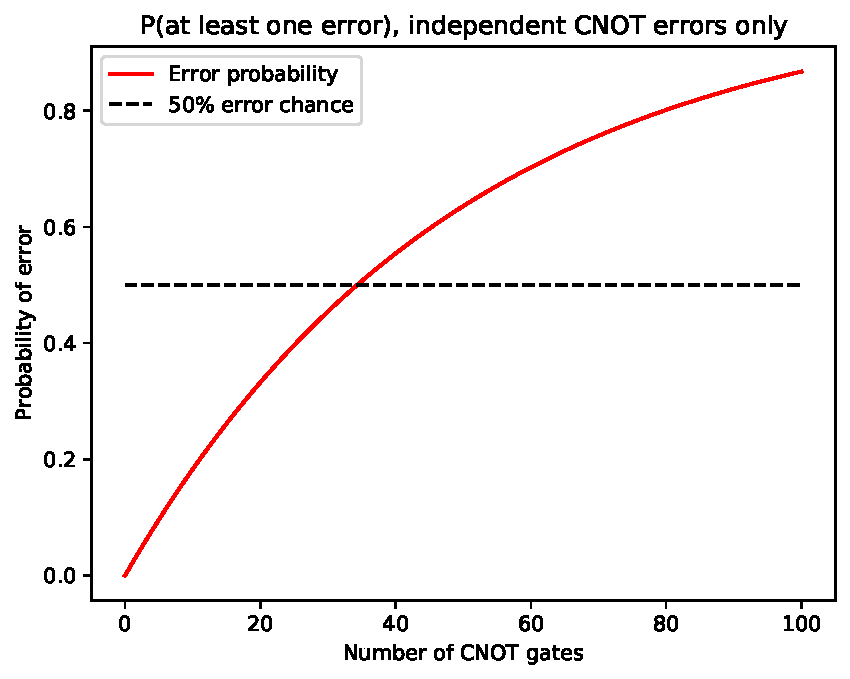
\includegraphics[width=3in]{Error.pdf}  
  \caption{The CNOT error.}
  \label{fig:err}
\end{figure}

We see in \cref{fig:err} that we have a better than even chance of error with
40 CNOT gates; considering the single-qubit errors reduces the manageable depth
of our circuit even further. Thus, without implementing error correction, which
is beyond the scope of this project and likely requires more than the five
qubits available on most of the Q Experience processors, we will limit our
circuit to fewer than 30 CNOT gates or so.

As mentioned in the previous paragraph, most public-facing IBM quantum
processors have five qubits (one exception has sixteen, but for a Hamiltonian
simulation limited to 30 CNOT gates it is too large to use effectively).
Furthermore, most of them are not arranged linearly, rather having a shape
like a T, which limits the Ising model to a maximum of four spins. We will use
all four available spins for our simulation.

As each implementation of $U(\Delta t)$ requires three CNOT gates, and three
applications of $U(\Delta t)$ are required to move four spins forward by one
unit of $\Delta t$, we will limit ourselves to three time evolution operations;
that is, $t_{max} = 3 \Delta t$. For our first computation suite, we take
$t = \frac12$.

\separator


%%%%%%%%%%%%%%%%%%%%%%%%%%%%%%%%%%%%%%%%%%%%%%%%%%%%%%%%%%%%%%%%%%%%%%%%%%%%%%%%
\subsection{Implementing time evolution} \label{subsec:implement}

Following the method and notation of \cite{Vatan2004}, our two-qubit Trotterized
time evolution operator is $N(-\Delta t, -\Delta t, -\Delta t)$. We can
implement it using with three CNOT gates as

\begin{figure}[ht]
  \centering
  \begin{equation*}
  \Qcircuit @C=1em @R=1.25em{
    & \multigate{1}{U(\Delta t)}  & \qw \\
    & \ghost{U(\Delta t)}         & \qw
  } \quad \equiv \quad
  \Qcircuit @C=1em @R=0.5em {
    & \qw                   & \targ     & \gate{R_z(-2 \Delta t - \frac\pi2)} 
      & \ctrl{1}  & \qw                               & \targ     
      & \gate{R_z(-\frac\pi2)}  & \qw \\
    & \gate{R_z(\frac\pi2)} & \ctrl{-1} & \gate{R_y(\frac\pi2 + 2 \Delta t)} 
      & \targ     & \gate{R_y(-2\Delta t - \frac\pi2)} & \ctrl{-1} 
      & \qw                     & \qw
  }
  \end{equation*}
  \caption{The quantum circuit for $U(\Delta t)$.}
  \label{fig:circuit}
\end{figure}

Note first that we implement the inverted CNOT gate, which gives the second and
sixth gates in \cref{fig:circuit}, as
\begin{equation*}
  \Qcircuit @C=1em @R=1.25em {
    & \targ     & \qw  \\
    & \ctrl{-1} & \qw 
  } \quad \equiv \quad
  \Qcircuit @C=1em @R=0.5em {
    & \gate{H} & \ctrl{1} & \gate{H} & \qw \\
    & \gate{H} & \targ    & \gate{H} & \qw
  } \quad ,
\end{equation*}
where $H$ is the Hadamard gate. Additionally, this construction neglects a global
phase of $e^{i\pi/4}$. However, we expect only to implement local observables, so
the global phase can be safely ignored; even if it could not, we could keep track
of it by hand to retain full information about our system.

As seen in \cref{fig:timecirc}, to approximately evolve our system in time by
$\Delta t$, we implement $U(\Delta t)$ on each pair of qubits in a cascading
sequence.

\begin{figure}[ht]
  \centering
  \begin{equation*}
  \Qcircuit @C=1em @R=0.5em {
  & \multigate{1}{U(\Delta t)}  & \qw                         & \qw     
    & \qw                         & \qw \\
  & \ghost{U(\Delta t)}         & \multigate{1}{U(\Delta t)}  & \qw     
    & \qw                         & \qw \\
  & \qw                         & \ghost{U(\Delta t)}         & \qw     
    & \qw                         & \qw \\
  &                             &                             & \ddots  
    &                             & \\
  &                             &                             &         
    &                             & \\
  & \qw                         & \qw                         & \qw     
    & \multigate{1}{U(\Delta t)}  & \qw \\
  & \qw                         & \qw                         & \qw     
    & \ghost{U(\Delta t)}         & \qw
  }
  \end{equation*}
  \caption{The Trotterized circuit for one increment of $\Delta t$.}
  \label{fig:timecirc}
\end{figure}

Finally, our full time evolution is obtained by repeating the entire circuit
of \cref{fig:timecirc} $n$ times (here, thrice).

\clearpage


%%%%%%%%%%%%%%%%%%%%%%%%%%%%%%%%%%%%%%%%%%%%%%%%%%%%%%%%%%%%%%%%%%%%%%%%%%%%%%%%
\section{Running the computation} \label{sec:run}
%%%%%%%%%%%%%%%%%%%%%%%%%%%%%%%%%%%%%%%%%%%%%%%%%%%%%%%%%%%%%%%%%%%%%%%%%%%%%%%%

We implement the Trotterized time evolution $(U(\frac12))^3$ approximating the
evolution to time $\frac32$ in increments $\Delta t = \frac12$ on the IBM
quantum computer \texttt{ibmq\_rome} and on the simulator
\texttt{qasm\_simulator}, which simulates the evolution in the absence of any
noise. We chose our particular processor for its fairly low CNOT error rate ---
its maximum two-qubit error is only 1.072\%. Running the computation on a more
error-prone processor, \texttt{ibmqx2}, gave abysmal results; nearly 75\% of the
computations evolving the ground state failed to preserve it. Both the real
computation and the simulation are averages of 1024 runs (called shots in
Qiskit).

Additionally, we simulated the \textit{exact} unitary time evolution, without
Trotterization, in Mathematica, to observe the error introduced by the Trotter
decomposition.

We implemented $U(\Delta t)$ on the following initial states:
\begin{enumerate}[label=(\roman*)]
  \item $\ket{0000}$, the ground state of the system;
  \item $\ket{\Psi} = \frac12 \sum_{x \in \{0,1\}^4} \ket{x}$, the uniform
        superposition over all basis states;
  \item $\ket{0101}$ and $\ket{1010}$, two singlet states with $S_{tot}^z = 0$;
  \item The highly entangled ``cluster state" $\ket{\Phi_C} 
        = \frac12\qty(\ket{0+0+} + \ket{+0-1} + \ket{-1-0} + \ket{-1+1})$,
        prepared according to the procedure given in 
        \cite{Jorrand2005}. Note that 
        $\ket{+} = \frac{1}{\sqrt{2}} \qty(\ket{0} + \ket{1})$, and that
        $\ket{-} = \frac{1}{\sqrt{2}} \qty(\ket{0} - \ket{1})$.
\end{enumerate}
The circuits for initialization are given in \cref{fig:init}. Note that Qiskit
automatically initializes qubits in the state $\ket{0000}$, so that required no
additional processing.

\begin{figure}[ht]
  \begin{subfigure}{0.4\textwidth}
    \centering
    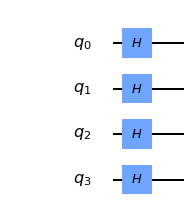
\includegraphics[height=1.25in]{init_unif.png}
    \subcaption{The circuit to initialize $\ket{\Psi}$.}
  \end{subfigure}
  \begin{subfigure}{0.4\textwidth}
    \centering
    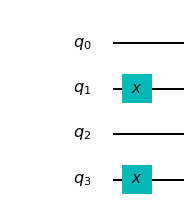
\includegraphics[height=1.25in]{init_sing_one.png}
    \subcaption{The circuit to initialize $\ket{0101}$.}
  \end{subfigure}
  
  \begin{subfigure}{0.4\textwidth}
    \centering
    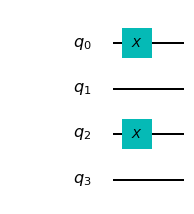
\includegraphics[height=1.25in]{init_sing_two.png}
    \subcaption{The circuit to initialize $\ket{1010}$.}
  \end{subfigure}
  \begin{subfigure}{0.4\textwidth}
    \centering
    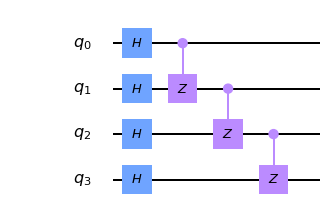
\includegraphics[height=1.25in]{init_clust.png}
    \subcaption{The circuit to initialize $\ket{\Phi_C}$.}
  \end{subfigure}
  \caption{The initialization circuits}
  \label{fig:init}  
\end{figure}

In \cref{fig:circuit}, we give the Qiskit circuit representation of
$U(\Delta t)$ and of our time evolution circuit acting on the prescribed
initial state.

\begin{figure}[ht]
  \begin{subfigure}{0.7\textwidth}
    \centering
    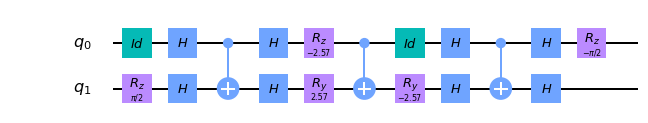
\includegraphics[width=\linewidth]{circ_Udt.png}
    \subcaption{The circuit implementing $U(\Delta t)$.}  
  \end{subfigure}
  
  \begin{subfigure}{0.9\textwidth}
    \centering
    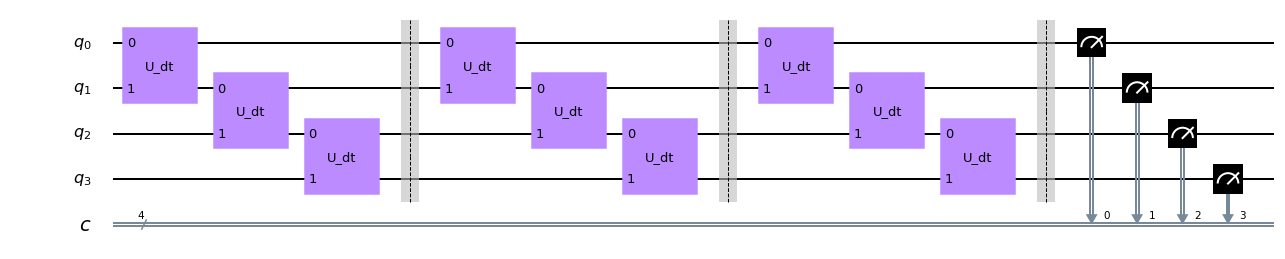
\includegraphics[width=\linewidth]{circ_timeEv.png}
    \subcaption{The circuit implementing time evolution on $\ket{0000}$.}  
  \end{subfigure}
  \caption{The circuit diagrams from Qiskit.}
  \label{fig:circ}
\end{figure}
%%%%%%%%%%%%%%%%%%%%%%%%%%%%%%%%%%%%%%%%%%%%%%%%%%%%%%%%%%%%%%%%%%%%%%%%%%%%%%%%
Finally, in \cref{fig:output}, we give histograms of the outputs. On the left
are the Q Experience histograms, which compare the real quantum computer to the
classical simulator; on the right are the Mathematica histograms giving the
exact outputs without Trotter error. The code used to generate them is included
in separate files with this report, but we regret that the download feature for
the Jupyter notebooks on IBM's Q Experience was not working, so that code
is included only as a series of screenshots.

\begin{figure}[hbt]
  \begin{subfigure}{0.4\textwidth}
    \centering
    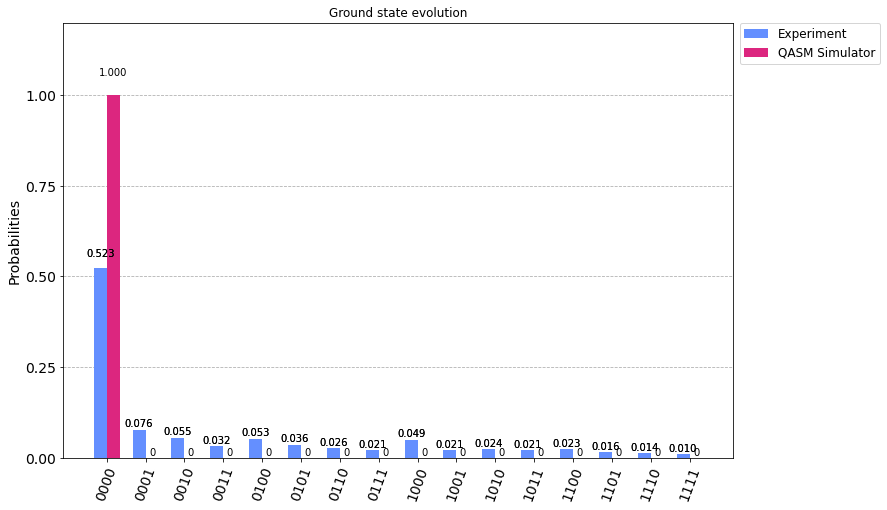
\includegraphics[width=0.9\linewidth]{input0_quantum.png}
    \subcaption{The quantum output from $\ket{0000}$.}
  \end{subfigure}
  \begin{subfigure}{0.4\textwidth}
    \centering
    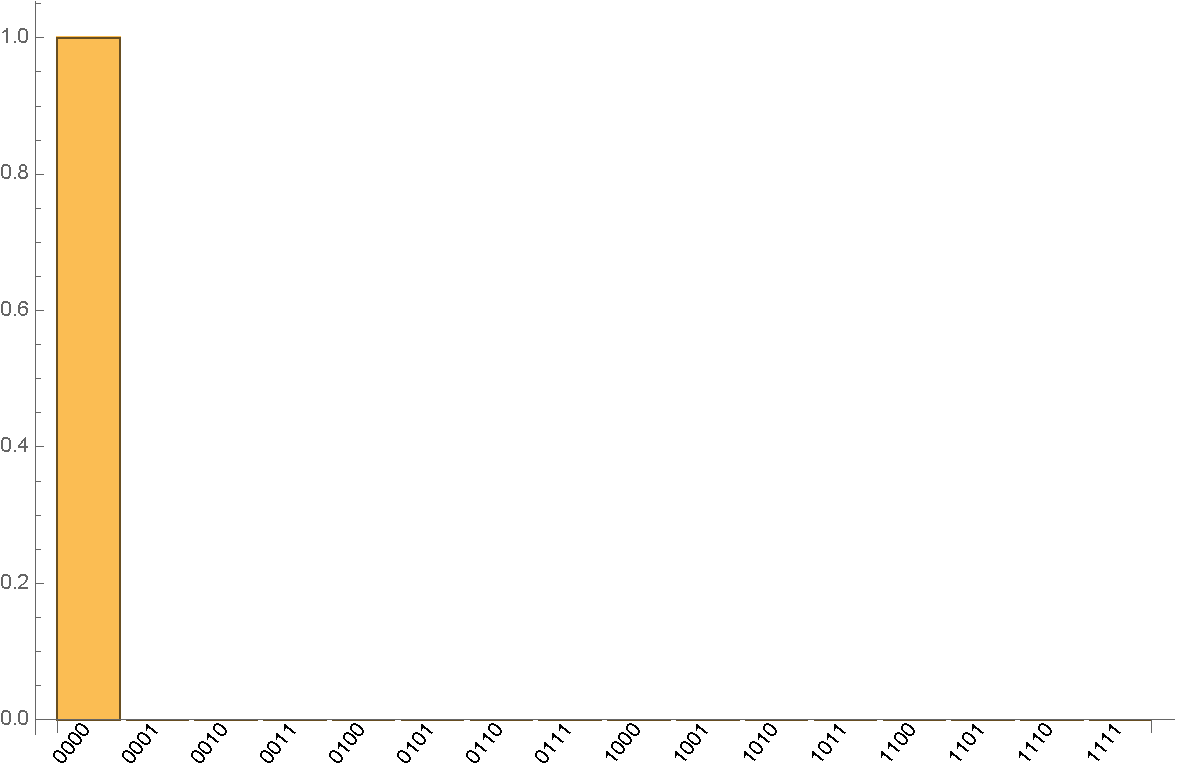
\includegraphics[width=0.9\linewidth]{input0_exact.pdf}
    \subcaption{The exact output from $\ket{0000}$.}  
  \end{subfigure}
  
    \begin{subfigure}{0.4\textwidth}
    \centering
    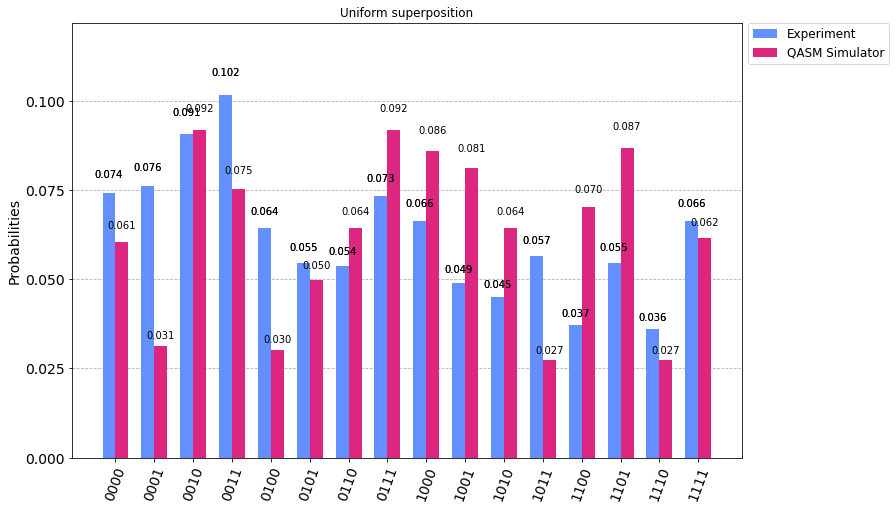
\includegraphics[width=0.9\linewidth]{inputUnif_quantum.png}
    \subcaption{The quantum output from $\ket{\Psi}$.}
  \end{subfigure}
  \begin{subfigure}{0.4\textwidth}
    \centering
    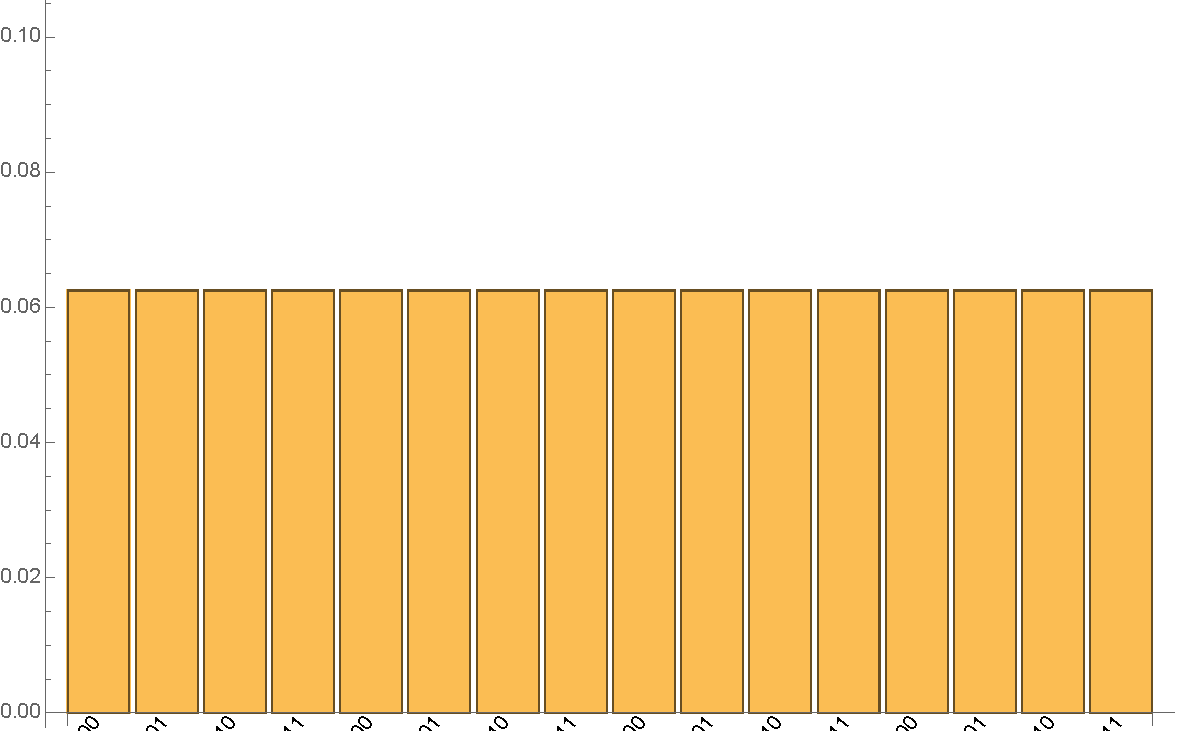
\includegraphics[width=0.9\linewidth]{inputUnif_exact.pdf}
    \subcaption{The exact output from $\ket{\Psi}$.}  
  \end{subfigure}
  
    \begin{subfigure}{0.4\textwidth}
    \centering
    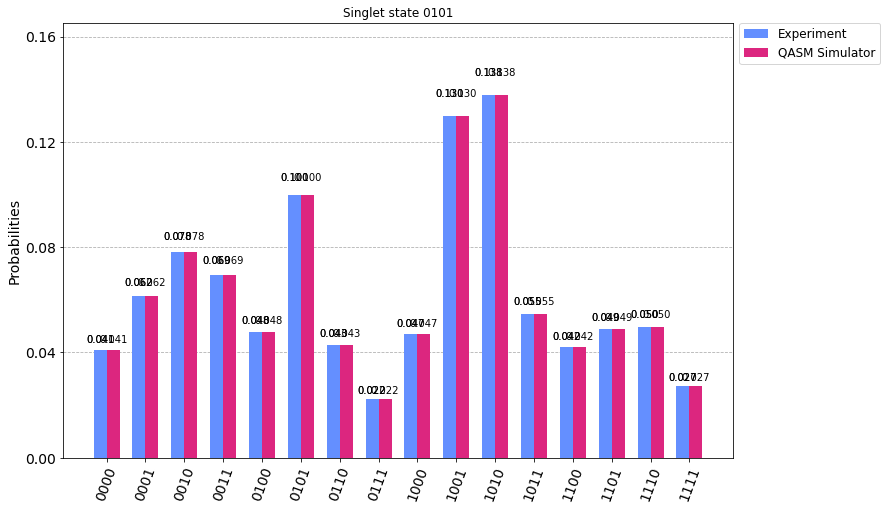
\includegraphics[width=0.9\linewidth]{inputSing1_quantum.png}
    \subcaption{The quantum output from $\ket{0101}$.}
  \end{subfigure}
  \begin{subfigure}{0.4\textwidth}
    \centering
    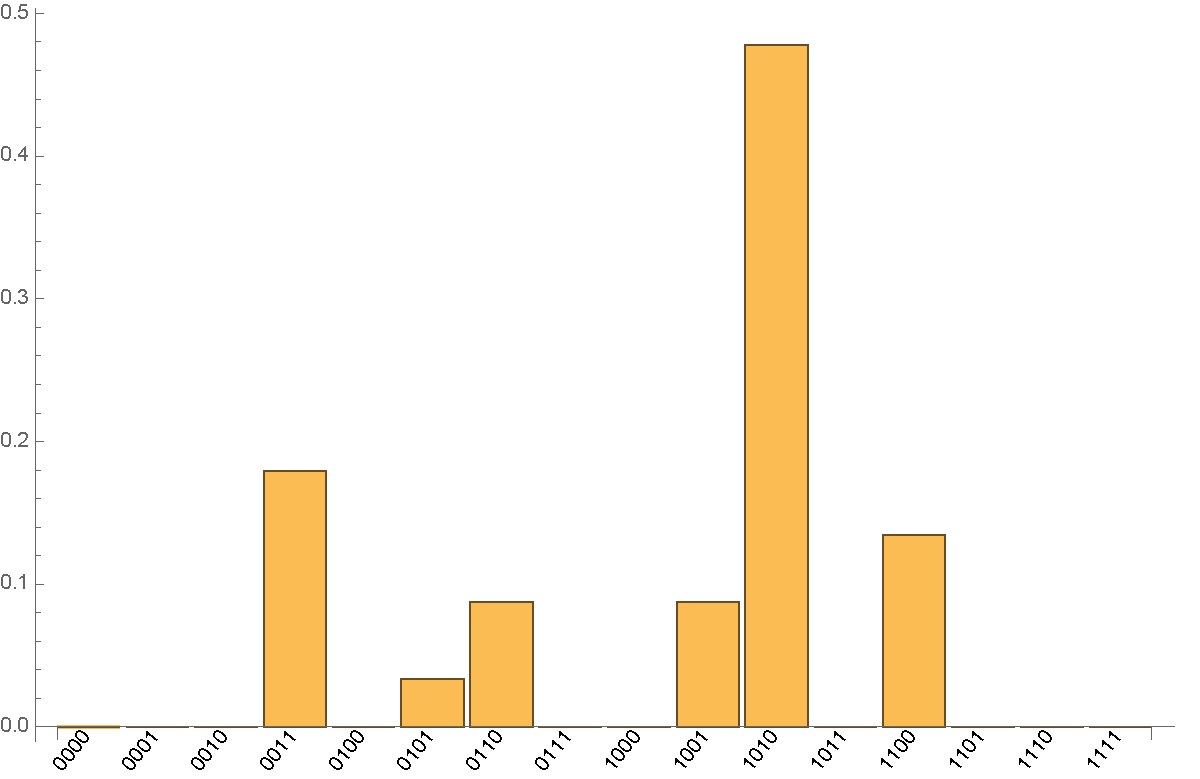
\includegraphics[width=0.9\linewidth]{inputSing1_exact.pdf}
    \subcaption{The exact output from $\ket{0101}$.}  
  \end{subfigure}
  
    \begin{subfigure}{0.4\textwidth}
    \centering
    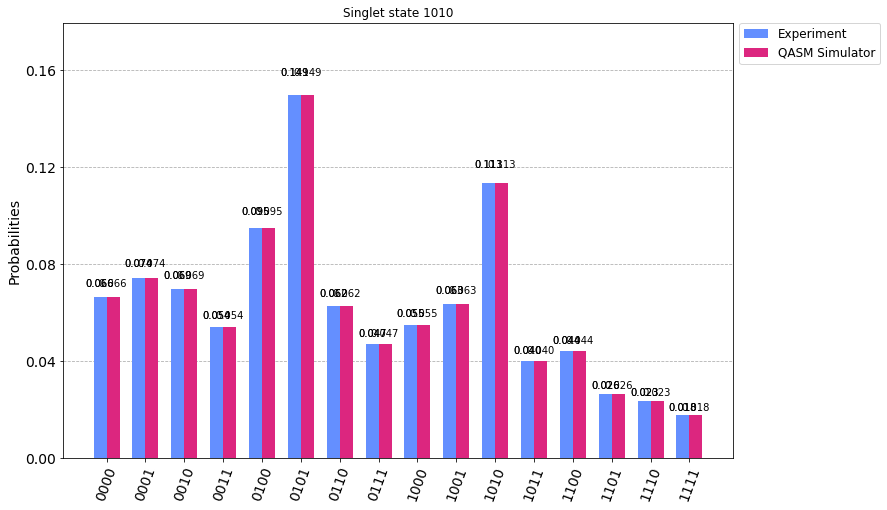
\includegraphics[width=0.9\linewidth]{inputSing2_quantum.png}
    \subcaption{The quantum output from $\ket{1010}$.}
  \end{subfigure}
  \begin{subfigure}{0.4\textwidth}
    \centering
    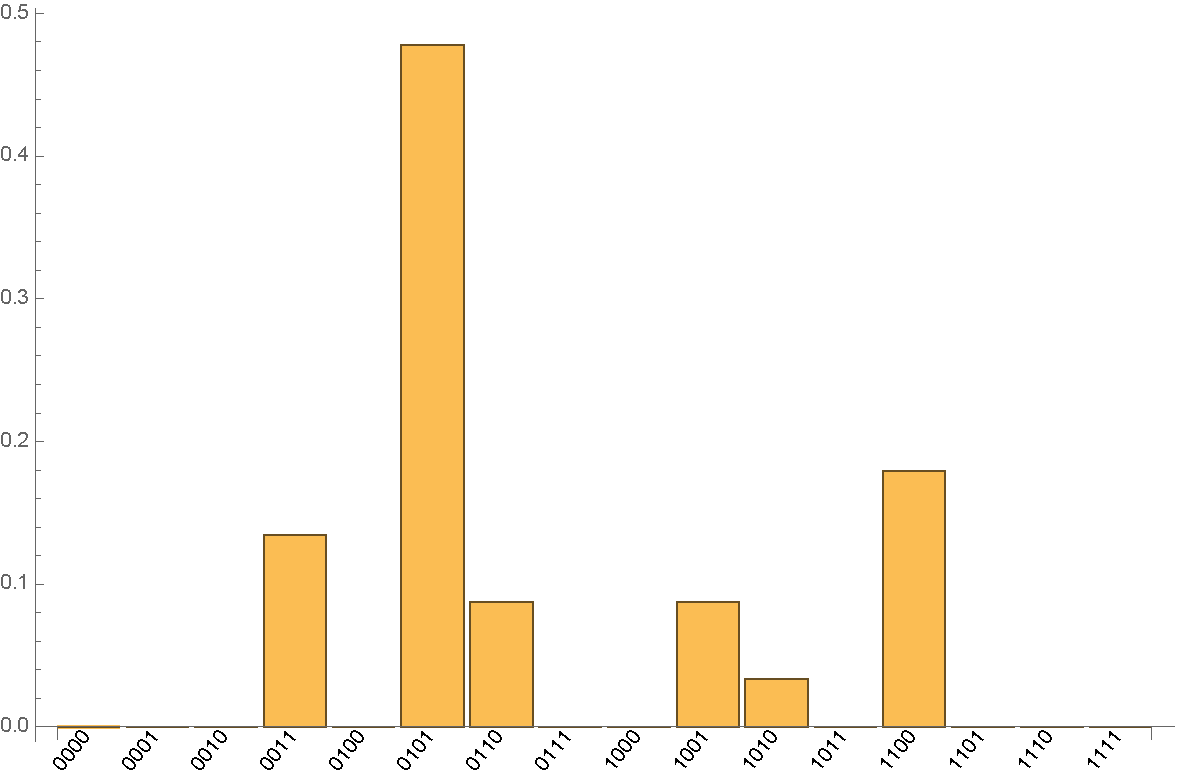
\includegraphics[width=0.9\linewidth]{inputSing2_exact.pdf}
    \subcaption{The exact output from $\ket{1010}$.}  
  \end{subfigure}
  
    \begin{subfigure}{0.4\textwidth}
    \centering
    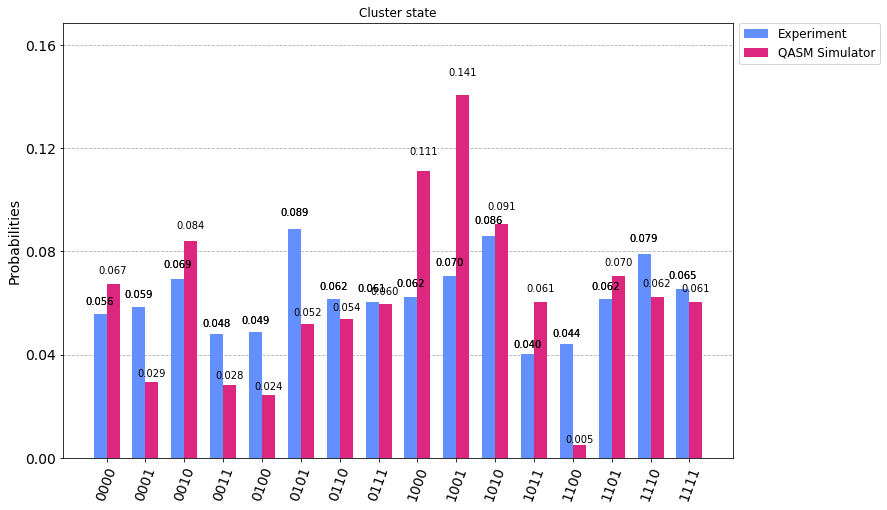
\includegraphics[width=0.9\linewidth]{inputClust_quantum.png}
    \subcaption{The quantum output from $\ket{\Phi_C}$.}
  \end{subfigure}
  \begin{subfigure}{0.4\textwidth}
    \centering
    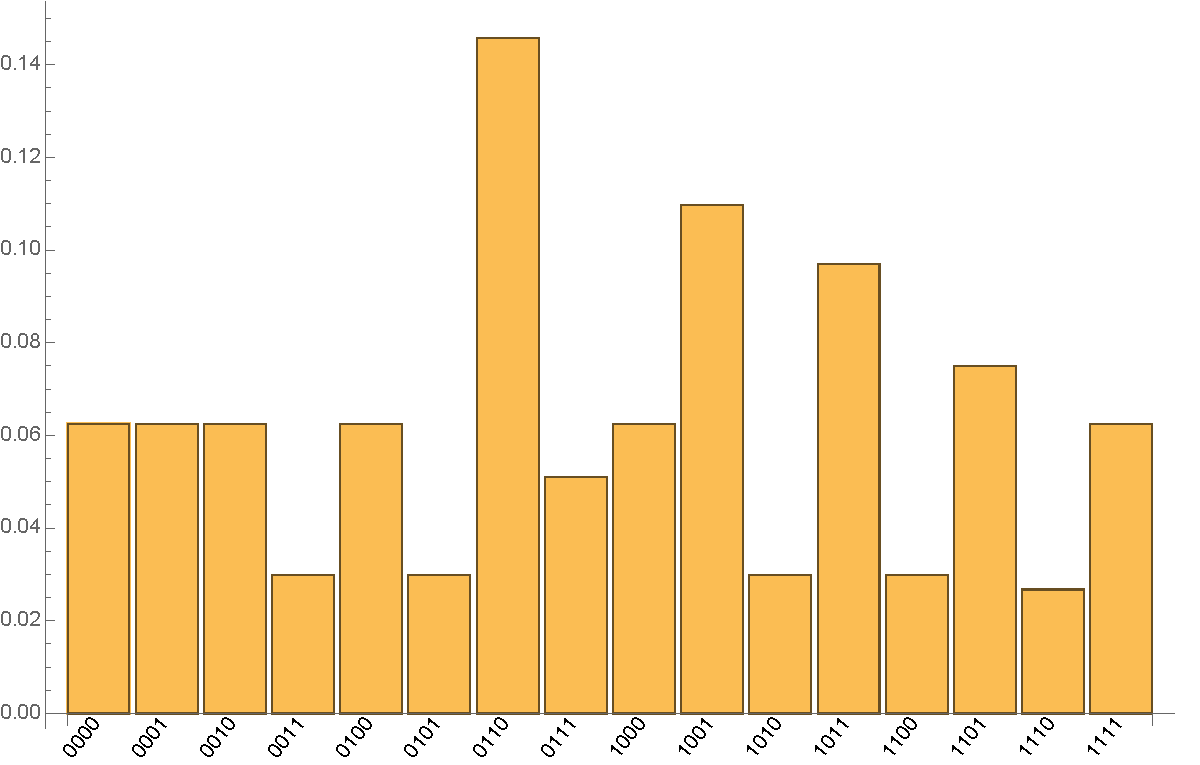
\includegraphics[width=0.9\linewidth]{inputClust_exact.pdf}
    \subcaption{The exact output from $\ket{\Phi_C}$.}  
  \end{subfigure}
  \caption{The output for $U(\Delta t = \frac12)^3$.}
  \label{fig:output}
\end{figure}

\clearpage 

Observing \cref{fig:output}, we may notice several things. The evolution of the
ground state $\ket{0000}$ is expected to preserve the state; both the exact
output and the simulated output replicate this behavior, but the real quantum
computation only maintains this 52.3\% of the time, even with our comparatively
short circuit.

When considering the uniform superposition state $\ket{\Psi}$, we may observe
that while the simulator and the true quantum computer do not agree very
closely, neither comes close to replicating the exact output, which preserves
$\ket{\Psi}$ (up to a global phase). Thus, Trotterization yields substantial
error in this case.

The output from the simulator and from \texttt{ibmq\_rome} agree almost exactly
when time evolving $\ket{0101}$ and $\ket{1010}$ in time, and they also both
preserve the dominance of the respective input state in the distribution of the
output. However, neither accurately predicts the second-most-likely output of
the exact evolution, nor do they maintain the expected zero probability of
the outputs not included in the exact result.

Finally, Trotter error is significant once more in the cluster state; the
simulator predicts the most probable outcome to be $\ket{1001}$, while the exact
outcome is most probably $\ket{0110}$. However, the noise in the quantum
processor is also significant, with the real quantum computer predicting
$\ket{0101}$ and $\ket{1010}$ to be the most likely outcomes (and with more
total variation overall, with only one of the sixteen outcomes having an
empirical probability of occuring below 0.04, while this is attained for five
outcomes in the exact output).

\separator


%%%%%%%%%%%%%%%%%%%%%%%%%%%%%%%%%%%%%%%%%%%%%%%%%%%%%%%%%%%%%%%%%%%%%%%%%%%%%%%%
\subsection{A run over a shorter time} \label{subsec:smallt}

We additionally conducted a run of the circuit, identical except that
$\Delta t = \frac{1}{100}$. This was designed to mostly remove the Trotter
error, allowing the quantum noise to shine through. The results of this are seen
in \cref{fig:smallt}.

\begin{figure}[hbt]
  \begin{subfigure}{0.4\textwidth}
    \centering
    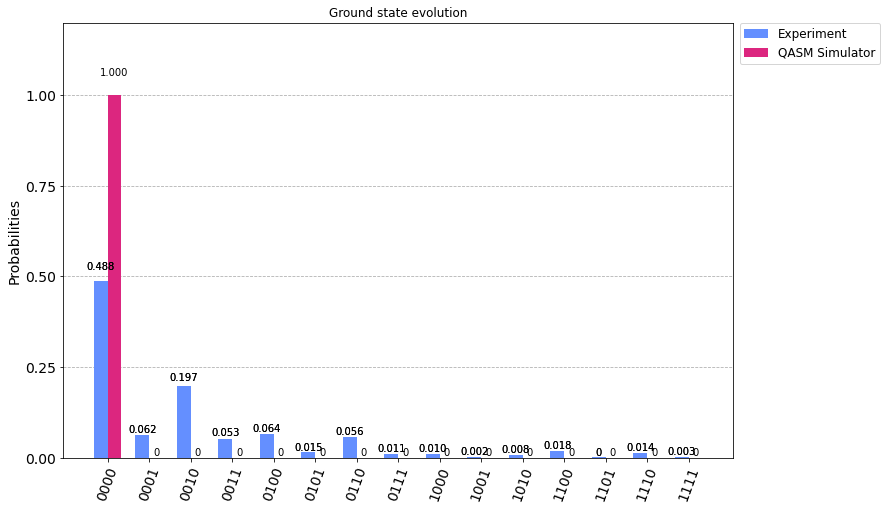
\includegraphics[width=0.9\linewidth]{smallt_input0_quantum.png}
    \subcaption{The quantum output from $\ket{0000}$.}
  \end{subfigure}
  \begin{subfigure}{0.4\textwidth}
    \centering
    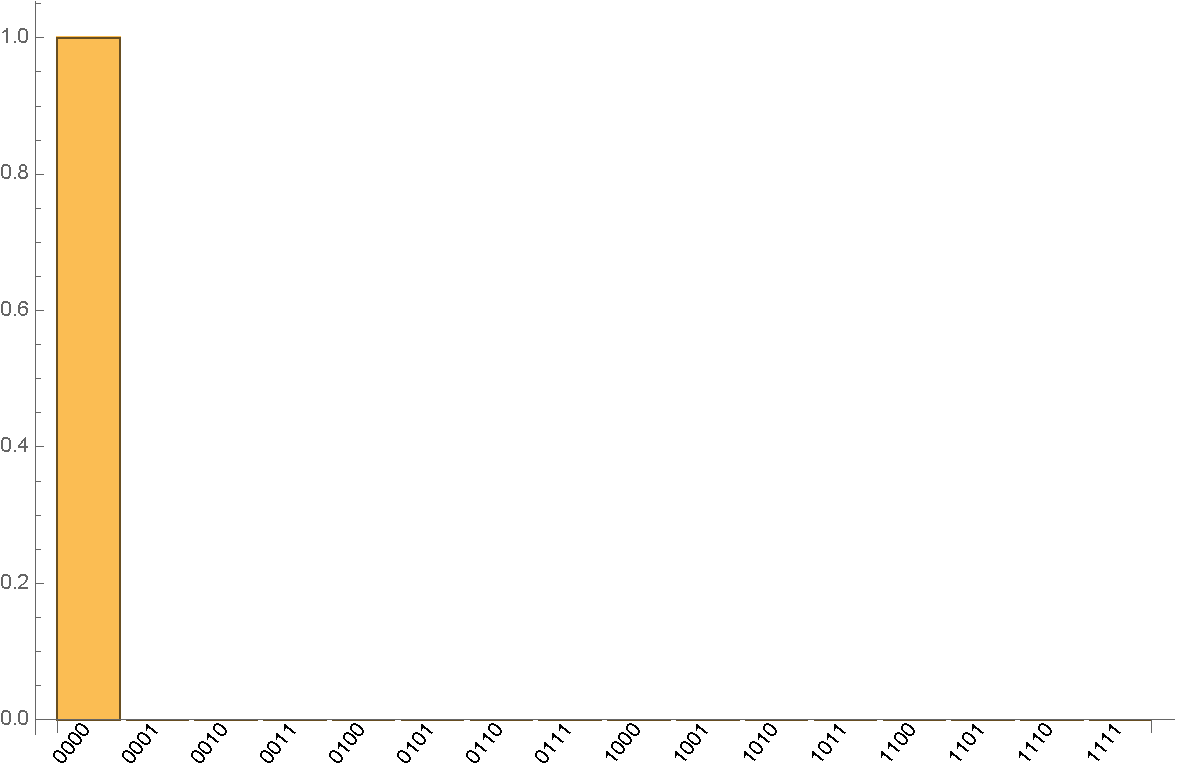
\includegraphics[width=0.9\linewidth]{smallt_input0_exact.pdf}
    \subcaption{The exact output from $\ket{0000}$.}  
  \end{subfigure}
  
    \begin{subfigure}{0.4\textwidth}
    \centering
    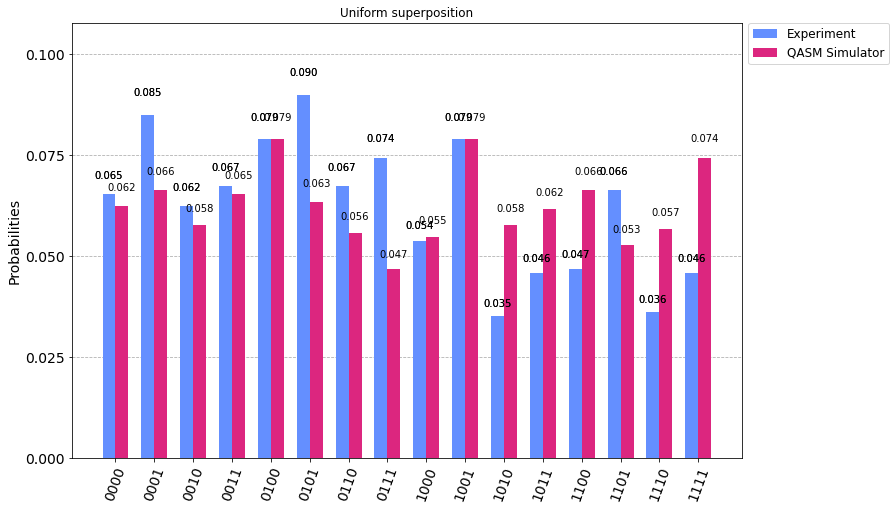
\includegraphics[width=0.9\linewidth]{smallt_inputUnif_quantum.png}
    \subcaption{The quantum output from $\ket{\Psi}$.}
  \end{subfigure}
  \begin{subfigure}{0.4\textwidth}
    \centering
    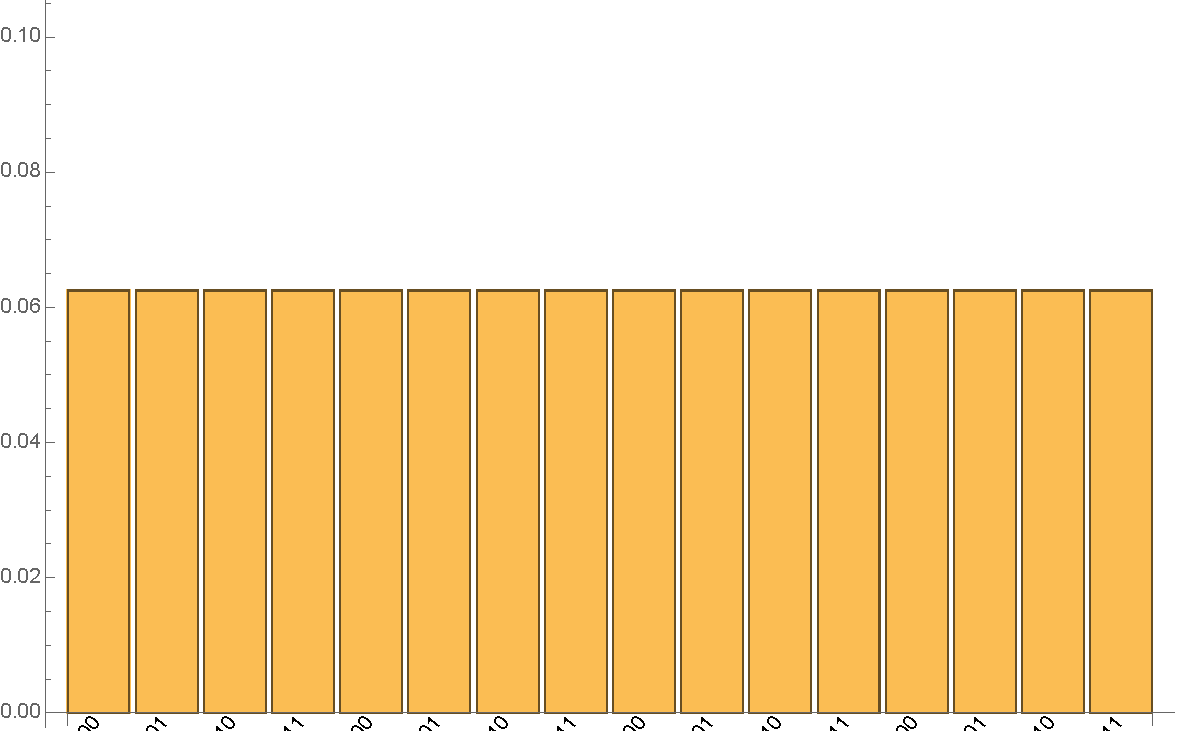
\includegraphics[width=0.9\linewidth]{smallt_inputUnif_exact.pdf}
    \subcaption{The exact output from $\ket{\Psi}$.}  
  \end{subfigure}
  
    \begin{subfigure}{0.4\textwidth}
    \centering
    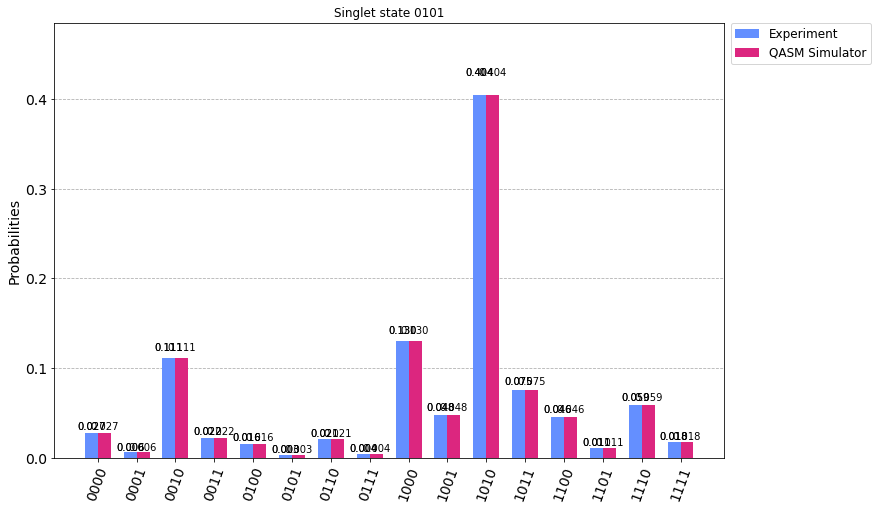
\includegraphics[width=0.9\linewidth]{smallt_inputSing1_quantum.png}
    \subcaption{The quantum output from $\ket{0101}$.}
  \end{subfigure}
  \begin{subfigure}{0.4\textwidth}
    \centering
    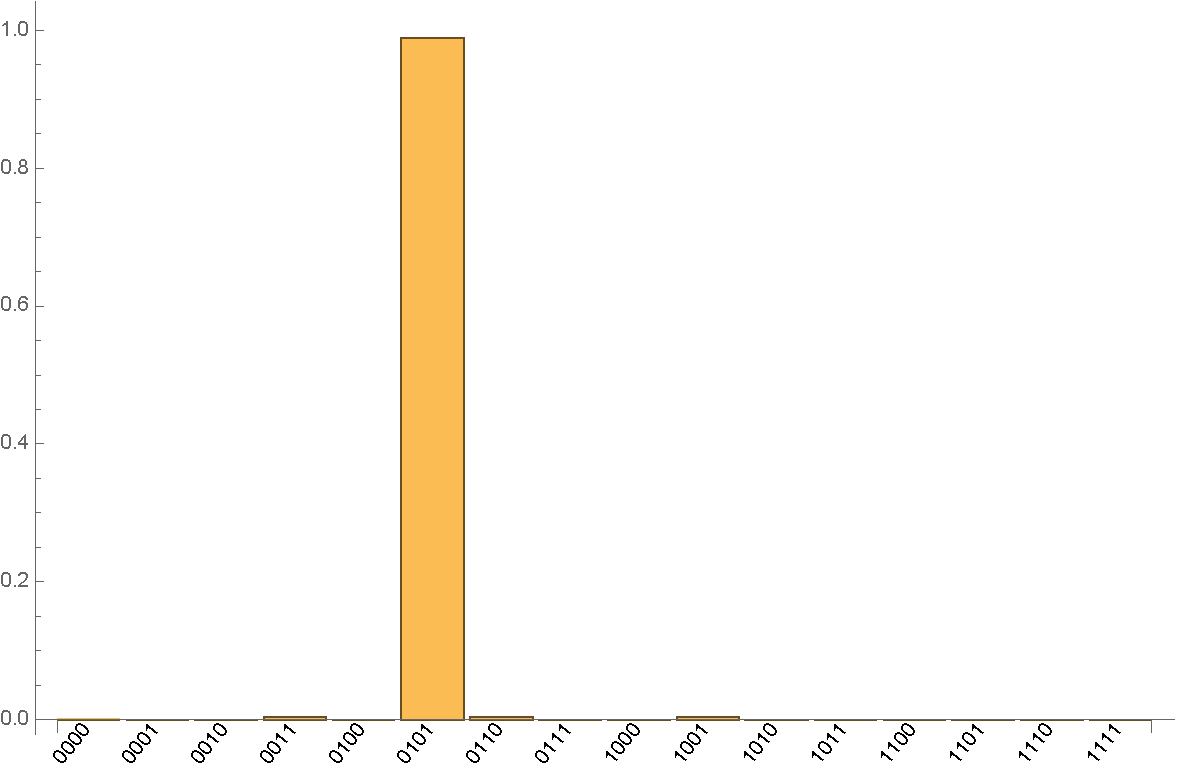
\includegraphics[width=0.9\linewidth]{smallt_inputSing1_exact.pdf}
    \subcaption{The exact output from $\ket{0101}$.}  
  \end{subfigure}
  
    \begin{subfigure}{0.4\textwidth}
    \centering
    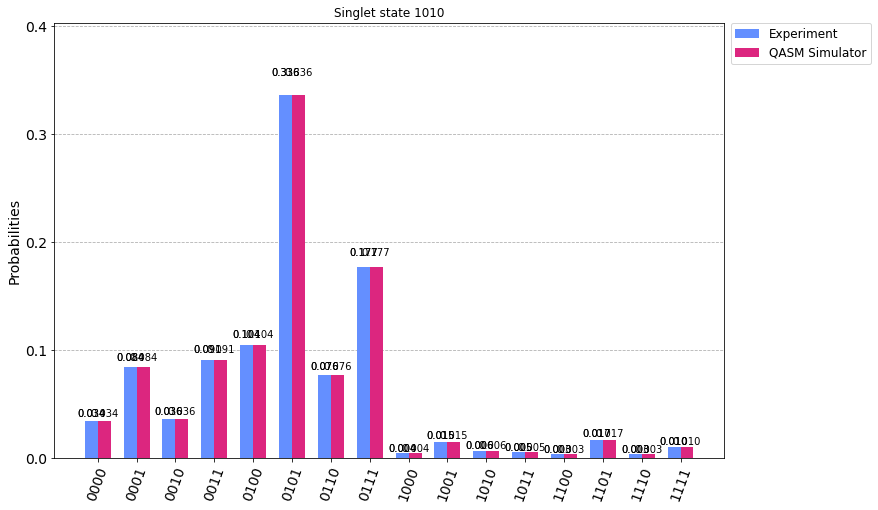
\includegraphics[width=0.9\linewidth]{smallt_inputSing2_quantum.png}
    \subcaption{The quantum output from $\ket{1010}$.}
  \end{subfigure}
  \begin{subfigure}{0.4\textwidth}
    \centering
    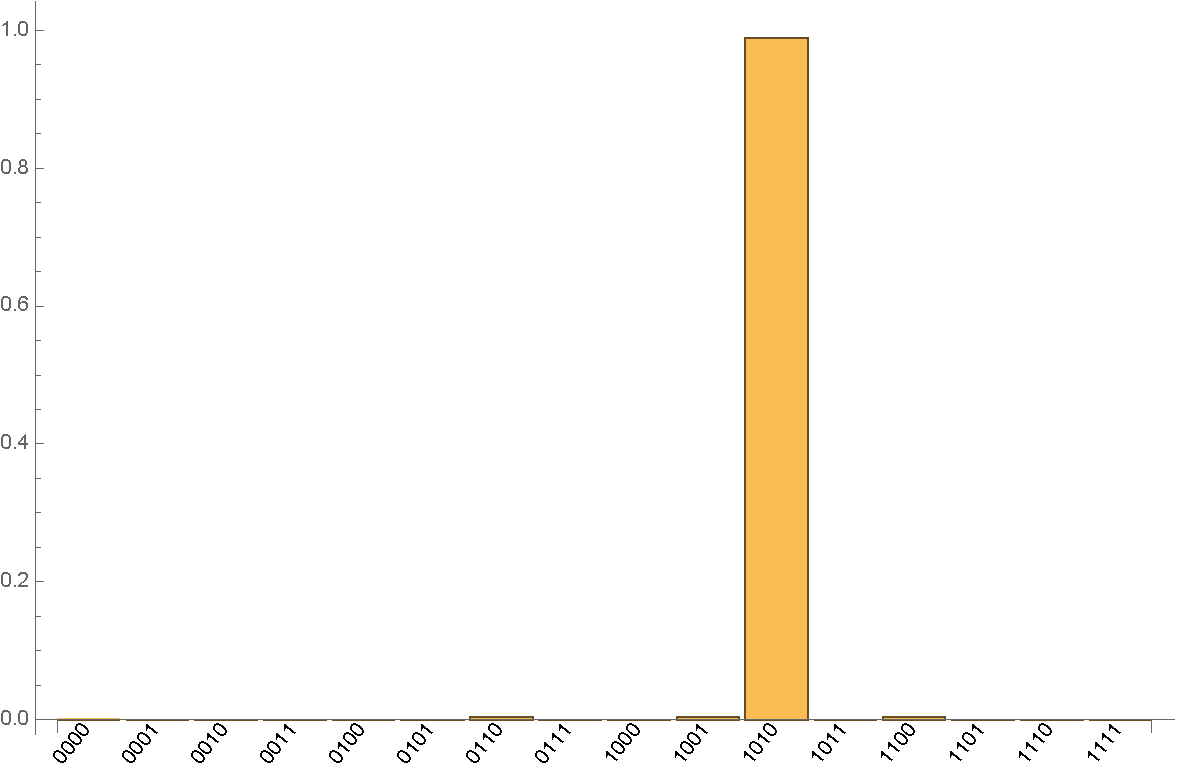
\includegraphics[width=0.9\linewidth]{smallt_inputSing2_exact.pdf}
    \subcaption{The exact output from $\ket{1010}$.}  
  \end{subfigure}
  
    \begin{subfigure}{0.4\textwidth}
    \centering
    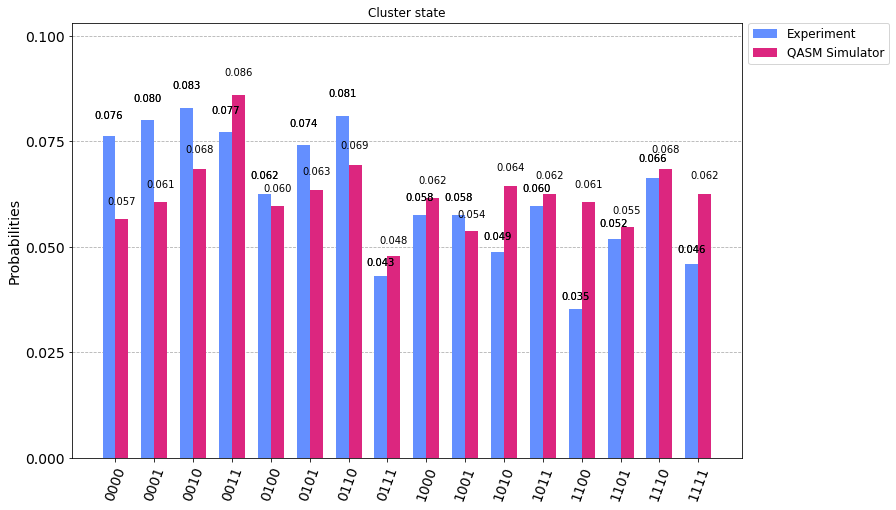
\includegraphics[width=0.9\linewidth]{smallt_inputClust_quantum.png}
    \subcaption{The quantum output from $\ket{\Phi_C}$.}
  \end{subfigure}
  \begin{subfigure}{0.4\textwidth}
    \centering
    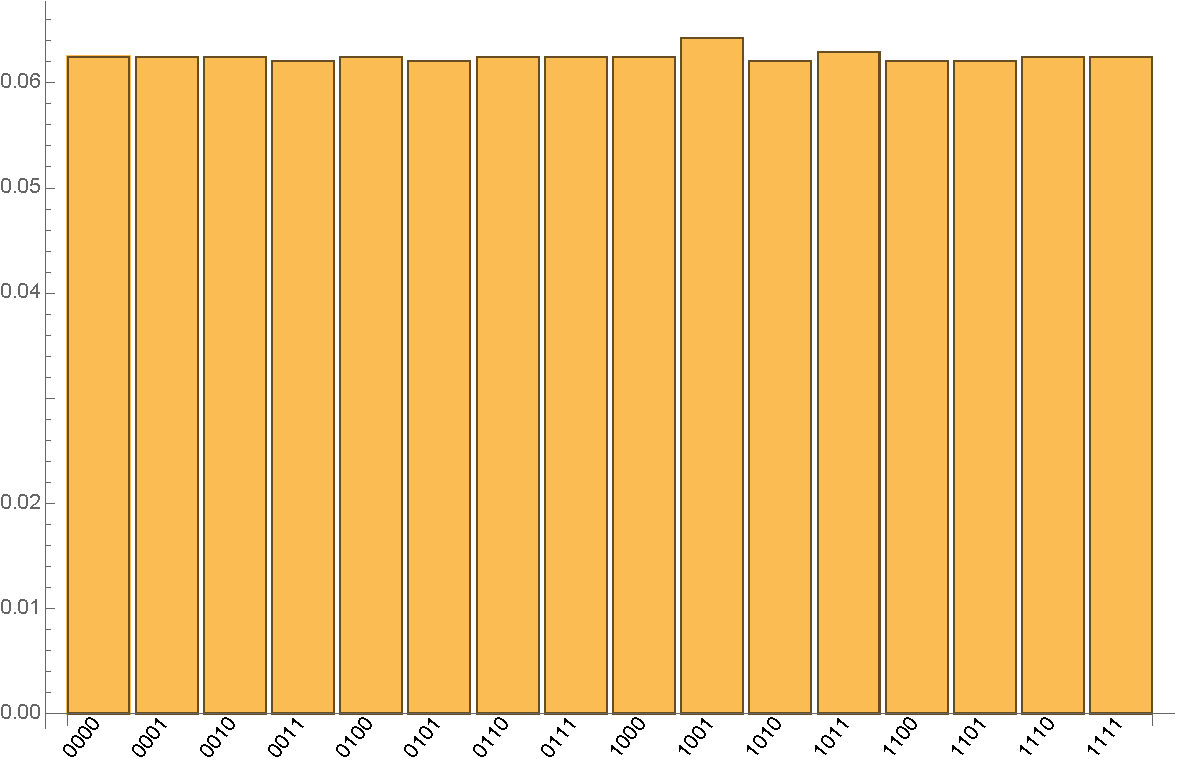
\includegraphics[width=0.9\linewidth]{smallt_inputClust_exact}
    \subcaption{The exact output from $\ket{\Phi_C}$.}  
  \end{subfigure}
  \caption{The output for $U(\Delta t = \frac{1}{100})^3$.}
  \label{fig:smallt}
\end{figure}

The noise is obviously apparent in the output for the ground state; the
probability of error in \texttt{ibmq\_rome} is still around $\frac12$. The
Trotter error is still somewhat visible, as $\ket{\Psi}$ is still not an
eigenstate, although some of the variation is explainable due to the finite
sample size (of 1024). The noise in the real computation increases this
variance as well. Nevertheless, the simulation has all probabilities between
approximately 0.047 and 0.079, not too far off from the exact 0.0625.

Comparing the singlet-state outputs from \cref{fig:output} and
\cref{fig:smallt}, an interesting note is made. In the exact solution when
$t_{final} = 0.03$, very little time has passed, so the output state is 
measured to be equal to the input with high probability; on the other hand,
after 1.5 time units, it is more likely that $\ket{0101} \mapsto \ket{1010}$ and
vice versa. When Trotterization is performed, however, both time steps give a
larger weight to the reversed singlet than to the initial state. Indeed, when
$\Delta t = 0.01$, neither the experimental nor the simulated Trotterized value
have a significant probability of finding $\ket{0101}$ or $\ket{1010}$ in their
respective initial states at all! This indicates that, even with such a small
time step, the first-order Trotterization scheme is too ``harsh" of an
evolution; a higher-order decomposition might be required to smooth out the
evolution of the Heisenberg chain.

Finally, the cluster state output is close to uniform in the exact description,
with some asymmetry beginning to show in the probabilities; the noise in both
the simulated and experimental quantum result overwhelms this subtle distinction
and makes it impossible to discuss the result in comparison.

\separator


%%%%%%%%%%%%%%%%%%%%%%%%%%%%%%%%%%%%%%%%%%%%%%%%%%%%%%%%%%%%%%%%%%%%%%%%%%%%%%%%
\subsection{Error analysis} \label{subsec:truerr}

Consider our independent error model of \cref{subsec:err}. Given the maximum
CNOT error rate of 0.0172 in \texttt{ibmq\_rome}, let us compare our observed
error rate over our two runs with the model. We consider the ground state (which
is preserved in the absence of noise) to produce this model.

Over 1024 shots, we correctly measured $\ket{0000}$ 52.3\% of the time,
indicating that 536 of the experiments completed with no errors. The second
experiment ran correctly 48.8\% of the time, indicative of precisely 500
correctly terminating experiments. On average, then, 518 experiments ran
without error, for an error rate of $1 - 0.5059 = 0.4941$.

Now, our circuit has a maximum number of 27 CNOT gates acting on any one qubit:
three from each implementation of $U(\Delta t)$, which acts a total of nine
times on the two central qubits. Our independent-CNOT-error model thus gives
a predicted error rate of $1 - (1 - 0.0172)^{27} = 1 - 0.6260 = 0.3740$, a
rather lower error rate than was observed. While our confidence in the actual
error rate of our circuit is not very high given only two trials, the
discrepancy is large enough that the highly na\"ive error model we propose is
probably not sufficient to characterize the error in a circuit of even modest
depth. More sophisticated treatments of the error will consider correlations
between errors, the single-qubit error rates, the decoherence time of the whole
circuit (by which errors become more likely as more gates are applied in
sequence), and even error in measurement.


\clearpage


%%%%%%%%%%%%%%%%%%%%%%%%%%%%%%%%%%%%%%%%%%%%%%%%%%%%%%%%%%%%%%%%%%%%%%%%%%%%%%%%
\section{Conclusions} \label{sec:conclusion}
%%%%%%%%%%%%%%%%%%%%%%%%%%%%%%%%%%%%%%%%%%%%%%%%%%%%%%%%%%%%%%%%%%%%%%%%%%%%%%%%

The most important conclusion we may draw from this study is the power of noise
to destroy quantum computational results and the consequent importance of
quantum error correction. Even in this circuit, for which no more than 
sixty-nine gates act upon any qubit (eleven gates in $U(\Delta t)$, which acts
six times in total on the two central qubits, and three more if initializing
$\ket{\Phi_C}$), the noise qualitatively changes the outcome of the circuit
relative to the noiseless simulator.

Even the Trotter error refers back to the noise; it is $\Ord(\Delta t^2)$,
indicating that our $\Delta t = \frac12$ is too large. However, the fact that
errors are so ubiquitous in the quantum computation means that we cannot run
more applications of $U(\Delta t)$ with a smaller time step to decrease the
overall error: while the Trotter error decreases, the error from decoherence
will increase apace, rendering our results just as useless. Likewise, the fact
that the eigenstates of the exact Hamiltonian are not always conserved under
Trotterization introduces error even for small values of $\Delta t$, requiring
better approximations to $e^{-i H t}$ to remedy.

Thus we see that, even for this simple system, quantum computers are not yet
ready to take on their classical counterparts in simulating many-body quantum
dynamics.


%%%%%%%%%%%%%%%%%%%%%%%%%%%%%%%%%%%%%%%%%%%%%%%%%%%%%%%%%%%%%%%%%%%%%%%%%%%%%%%%
\subsection{Further direction} \label{subsec:further}

It is worth mentioning, however, that the algorithm described above is quite
flexible. Following the method of \cite{Vatan2004}, $U(\Delta t)$ could be
modified to apply to the general XYZ spin chain, which has Hamiltonian
\[
  H_{XYZ} = \Sum_{i=1}^{L-1} \qty[\alpha \sigma_i^x \sigma_{i+1}^x 
        + \beta \sigma_i^y \sigma_{i+1}^y + \gamma \sigma_i^z \sigma_{i+1}^z],
\]
by simply altering the parameters in the Pauli rotation gates. Depending on the
connectivity of the quantum circuit, periodic boundary conditions could also be
implemented, although in the case of the IBM Q Experience processors would not
readily accept this modification.

Additionally, while we showed the effect of preparing different input states,
we could also measure various observables. Local observables would be relatively
straightforward to implement; we would need to rotate each qubit into the
observable's eigenbasis, then measure. For global observables, the quantum phase
estimation algorithm, which is described in \cite{NielsenChuang}, is utilized;
however, it requires an ancillary register of $k$ qubits if the given eigenvalue
is to be simulated with a precision of $2^{-k}$. This is not particularly
difficult to envision, but the five qubits available on most IBM processors are
not sufficient. The gate depth of this circuit is also larger than the Q
Experience processors could effectively handle.

\clearpage 

%%%%%%%%%%%%%%%%%%%%%%%%%%%%%%%%%%%%%%%%%%%%%%%%%%%%%%%%%%%%%%%%%%%%%%%%%%%%%%%%
\printbibliography

\end{document}